%! TeX root = gym_comm_obs_action_space.tex

\documentclass[tikz]{standalone}
\usetikzlibrary{positioning}
\usetikzlibrary{arrows.meta}
\usetikzlibrary{calc}
\tikzset{
    every node/.append style={very thick,rounded corners=0.1mm},
    service/.style={{Circle[green!50!black, length=6pt]}-Latex, thick, green!50!black,,shorten <=-3pt},
    action/.style={{Circle[blue!70!black,length=6pt]}-Latex, thick, blue!70!black, dashed,shorten <=-3pt},
    node/.style={fill=yellow!20, draw=yellow!50!black},
    y=0.7cm
}

\begin{document}
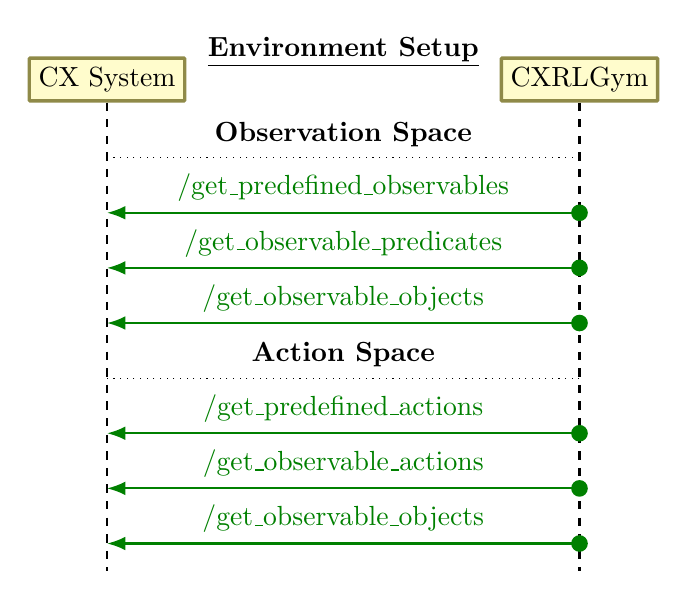
\begin{tikzpicture}
\node[node] (CX) at (0,0) {CX System};
\node[node] (Gym) at (6,0) {CXRLGym};
\node[] (desc) at (3,0.5) {\underline{\textbf{Environment Setup}}};

\draw[dashed, thick] (CX.south) -- ++(0,-8.5);
\draw[dashed, thick] (Gym.south) -- ++(0,-8.5);

\begin{scope}[shift={($(Gym.south)+(0,0)$)}]
\draw[dotted] (0,-1) -- ++(-6,0) node[midway, above] {\textbf{Observation Space}};
\draw[service] (0,-2) -- ++(-6,0) node[midway, above] {/get\_predefined\_observables};
\draw[service] (0,-3) -- ++(-6,0) node[midway, above] {/get\_observable\_predicates};
\draw[service] (0,-4) -- ++(-6,0) node[midway, above] {/get\_observable\_objects};
\draw[dotted] (0,-5) -- ++(-6,0) node[midway, above] {\textbf{Action Space}};
\draw[service] (0,-6) -- ++(-6,0) node[midway, above] {/get\_predefined\_actions};
\draw[service] (0,-7) -- ++(-6,0) node[midway, above] {/get\_observable\_actions};
\draw[service] (0,-8) -- ++(-6,0) node[midway, above] {/get\_observable\_objects};
\end{scope}
\end{tikzpicture}
\end{document}
